% !TEX root =./main.tex
\section{Block 2 : Time Gain Compensation}

As sound travels, it attenuates through geometric spreading.  As a result, the magnitude of the second reflected pulse is significantly lower. Therefore, the program must compensate to increase the magnitudes of the two pulses back to the original magnitude of 1. 
    The samples must first be converted into distance. This is easily accomplished using the following conversion.
    \begin{align*}
     \frac{\text{Sample Index}}{F_s} \cdot c_{\text{sound}}    
    \end{align*}
    

    Although the speaker has some degree of directivity, the best results were found using the inverse- square law $(I \propto  \frac{1} {r^2} )$. 

    \begin{figure}[H]
        \centering
        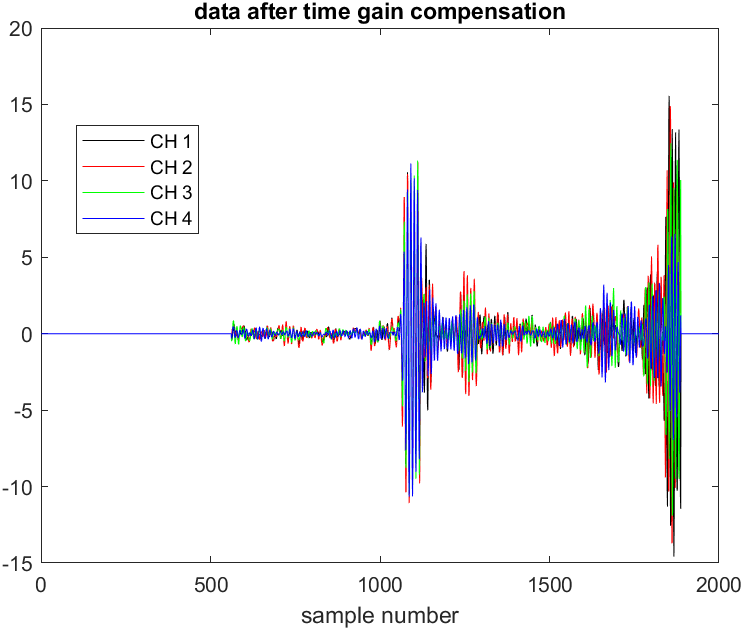
\includegraphics[width=0.5\linewidth]{figures/time_gain_1.png}
        \caption{Data after time gain compensation}
        \label{fig:time_gain1}
    \end{figure}

    \ref{fig:time_gain1}

